
\documentclass[11pt]{report}

\usepackage{graphicx}
%\graphicspath{ {images/} }

\marginparwidth 0.5in 
\oddsidemargin 0.25in 
\evensidemargin 0.25in 
\marginparsep 0.25in
\topmargin 0.0in 
\textwidth 6in \textheight 8.5in

\title{sQuire: A Web Based Collaborative Editor}
\author{bolt1003, wern0096, alsh5301, sass8427, dani2918, boss2849, snev7821, jank6275}

\begin{document}
\maketitle

\tableofcontents

\chapter{Application Domain Specification}

\section{Program Premise}
\begin{figure}[h!]
\caption{Squire will be a web-based collaborative text editor that compiles java code in throwaway "rooms". Multiple users can edit and communicate in real time.}
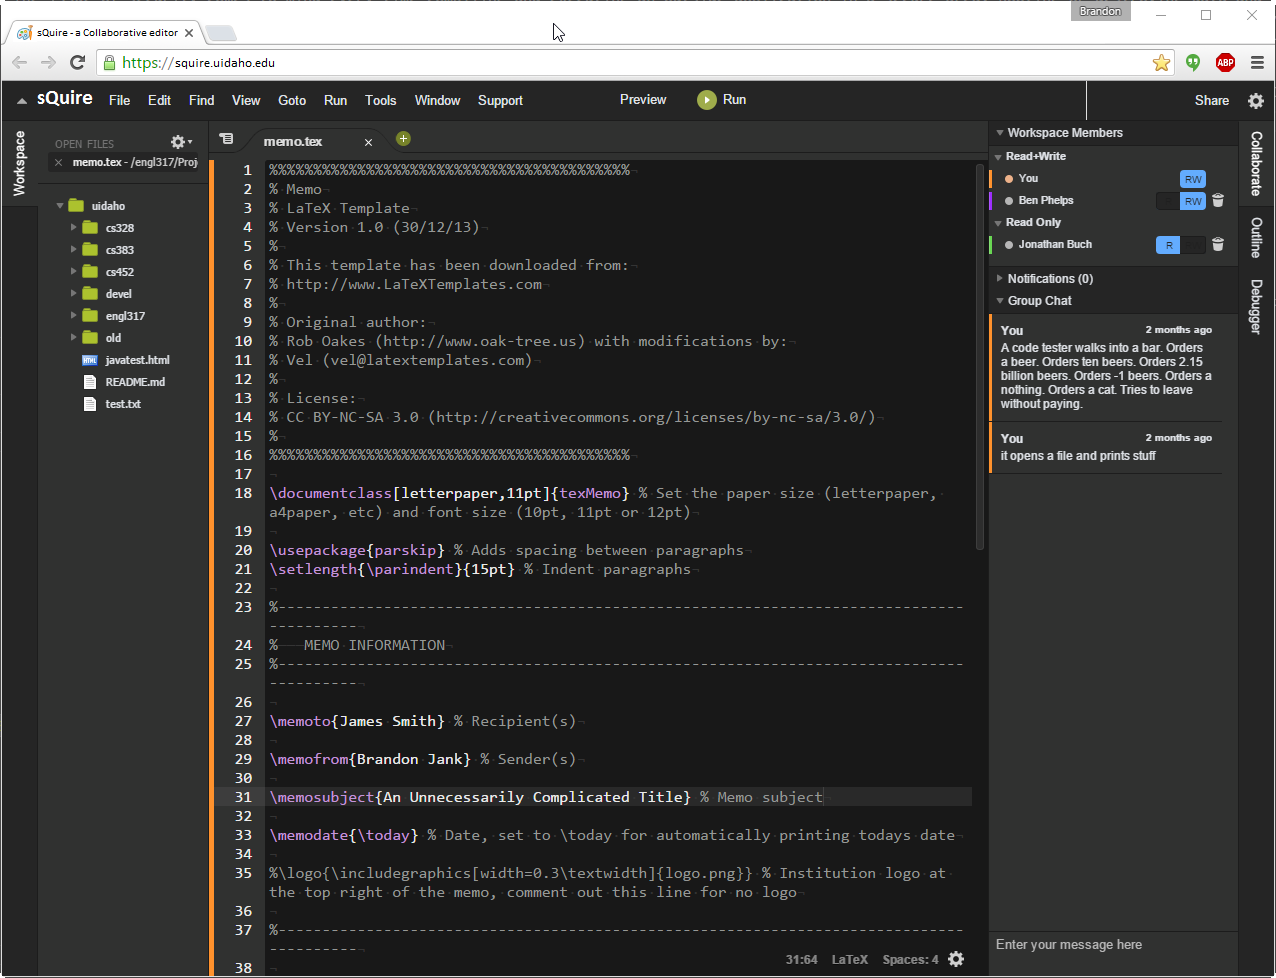
\includegraphics[width=0.7\textwidth]{squire}
\end{figure}



\section{Use Case Diagrams}
\subsection{Overview (jank6275)}
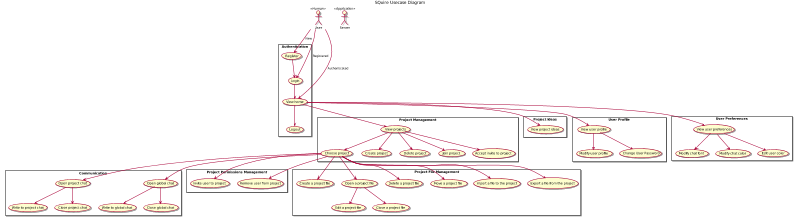
\includegraphics[width=0.7\textwidth]{diagrams/overview-jank6275}

\subsection{Project Ideas (dani2918)}
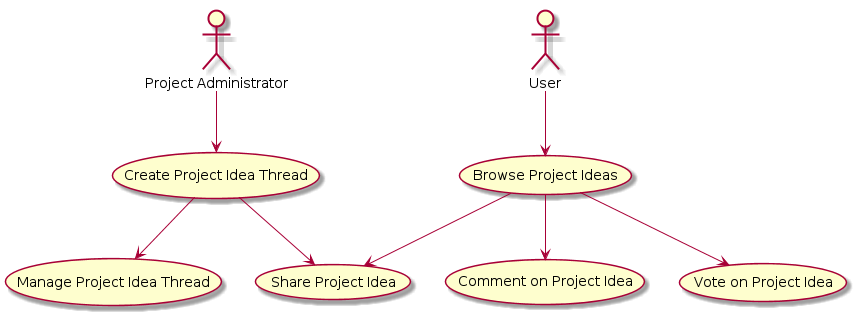
\includegraphics[width=0.7\textwidth]{diagrams/dani2918}

\subsection{Communication (jank6275)}
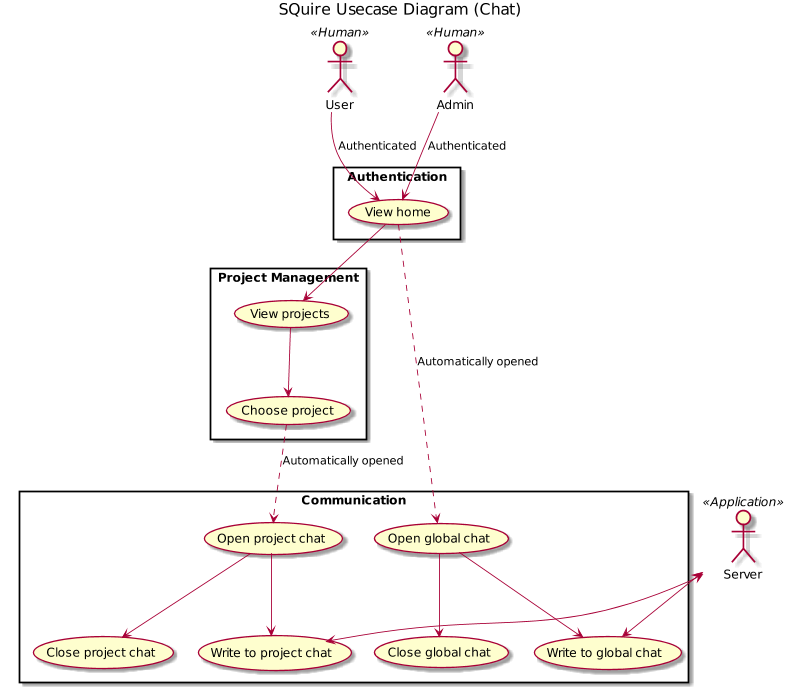
\includegraphics[width=0.7\textwidth]{diagrams/jank6275}



\section{Use Case Descriptions}

\subsection{Communication (jank6275)}
\subsubsection{Open project chat (jank6275)}
\begin{tabular}{ p{2cm} p{12cm} }
 \hline
 \\
 \textit{Actors:} & User \\ 
 \\
 \textit{Goals:} & To open the project chat window. \\
 \\
 \textit{Pre-conditions:} & User must be registered, signed in, and in editor Mode.  \\
 \\
 \textit{Summary:} & User clicks on open project chat and the chat opens, displaying chat history and updating when needed. \\ 
 \\
 \textit{Related use cases:} & Join global chat. \\ 
 \\
 \textit{Steps:} & \begin{enumerate}
  \item User clicks open project chat.
  \item Chat is notified that user has joined.
  \item System displays project chat window.
 \end{enumerate} \\
 \\
 \textit{Alternatives:} & None. \\
 \\
 \textit{Post-conditions:} & None. \\
 \\
\hline
\end{tabular}

\subsubsection{Open global chat (jank6275)}
\begin{tabular}{ p{2cm} p{12cm} }
 \hline
 \\
 \textit{Actors:} & User \\ 
 \\
 \textit{Goals:} & To open the global chat window. \\
 \\
 \textit{Pre-conditions:} & User must be registered, signed in, and anywhere on website.  \\
 \\
 \textit{Summary:} & User clicks on open global chat and the chat opens, displaying chat history and updating when needed. \\ 
 \\
 \textit{Related use cases:} & Join project chat. \\ 
 \\
 \textit{Steps:} & \begin{enumerate}
  \item User clicks open global chat.
  \item Chat is notified that user has joined.
  \item System displays global chat window.
 \end{enumerate} \\
 \\
 \textit{Alternatives:} & None. \\
 \\
 \textit{Post-conditions:} & None. \\
 \\
\hline
\end{tabular}

\subsubsection{Close project chat (jank6275)}
\begin{tabular}{ p{2cm} p{12cm} }
 \hline
 \\
 \textit{Actors:} & User \\ 
 \\
 \textit{Goals:} & To close the project chat window. \\
 \\
 \textit{Pre-conditions:} & User must be registered, signed in, and in editor Mode.  \\
 \\
 \textit{Summary:} & User clicks on close project chat and the chat window closes. \\ 
 \\
 \textit{Related use cases:} & Close global chat. \\ 
 \\
 \textit{Steps:} & \begin{enumerate}
  \item User clicks close project chat.
  \item Chat is notified that user has left.
  \item Client closes project chat window.
 \end{enumerate} \\
 \\
 \textit{Alternatives:} & None. \\
 \\
 \textit{Post-conditions:} & None. \\
 \\
\hline
\end{tabular}

\subsubsection{Close global chat (jank6275)}
\begin{tabular}{ p{2cm} p{12cm} }
 \hline
 \\
 \textit{Actors:} & User \\ 
 \\
 \textit{Goals:} & To close the global chat window. \\
 \\
 \textit{Pre-conditions:} & User must be registered, signed in, and anywhere on website.  \\
 \\
 \textit{Summary:} & User clicks on open global chat and the chat opens, displaying chat history and updating when needed. \\ 
 \\
 \textit{Related use cases:} & Close project chat. \\ 
 \\
 \textit{Steps:} & \begin{enumerate}
  \item User clicks close global chat.
  \item Chat is notified that user has left.
  \item Client closes global chat window.
 \end{enumerate} \\
 \\
 \textit{Alternatives:} & None. \\
 \\
 \textit{Post-conditions:} & None. \\
 \\
\hline
\end{tabular}

\subsubsection{Write to project chat (jank6275)}
\begin{tabular}{ p{2cm} p{12cm} }
 \hline
 \\
 \textit{Actors:} & User \\ 
 \\
 \textit{Goals:} & To send text to project chat. \\
 \\
 \textit{Pre-conditions:} & User must be registered, signed in, a project opened, with the project chat window open, and the text box selected.  \\
 \\
 \textit{Summary:} & User clicks in the project chat text box and then types a message then either presses enter or clicks the submit button. The text is displayed to all users in the chat, including the user. \\ 
 \\
 \textit{Related use cases:} & Write to global chat. \\ 
 \\
 \textit{Steps:} & \begin{enumerate}
  \item User clicks in the project chat box.
  \item User types a message and then presses enter or clicks submit button.
  \item Message is relayed to all clients with project chat open.
  \item Message is displayed.
 \end{enumerate} \\
 \\
 \textit{Alternatives:} & None. \\
 \\
 \textit{Post-conditions:} & None. \\
 \\
\hline
\end{tabular}

\subsubsection{Write to global chat (jank6275)}
\begin{tabular}{ p{2cm} p{12cm} }
 \hline
 \\
 \textit{Actors:} & User \\ 
 \\
 \textit{Goals:} & To send text to global chat. \\
 \\
 \textit{Pre-conditions:} & User must be registered, signed in, anywhere on website, with the global chat window open, and the text box selected.  \\
 \\
 \textit{Summary:} & User clicks in the global chat text box and then types a message then either presses enter or clicks the submit button. The text is displayed to all users in the chat, including the user. \\ 
 \\
 \textit{Related use cases:} & Write to project chat. \\ 
 \\
 \textit{Steps:} & \begin{enumerate}
  \item User clicks in the global chat box.
  \item User types a message and then presses enter or clicks submit button.
  \item Message is relayed to all clients with global chat open.
  \item Message is displayed.
 \end{enumerate} \\
 \\
 \textit{Alternatives:} & None. \\
 \\
 \textit{Post-conditions:} & None. \\
 \\
\hline
\end{tabular}

\subsubsection{Modify chat font (jank6275)}
\begin{tabular}{ p{2cm} p{12cm} }
 \hline
 \\
 \textit{Actors:} & User \\ 
 \\
 \textit{Goals:} & To change a users font style inside the global and project chat. \\
 \\
 \textit{Pre-conditions:} & User must be registered, signed in, the user settings window opened, and the chat settings tab open.  \\
 \\
 \textit{Summary:} & The user clicks the settings menu and changes their font style for both the project and global chat through a drop down box of available fonts. \\ 
 \\
 \textit{Related use cases:} & Modify chat color. \\ 
 \\
 \textit{Steps:} & \begin{enumerate}
  \item User clicks the settings menu.
  \item User clicks chat settings tab.
  \item User clicks chat font drop down box.
  \item User clicks desired font.
  \item User clicks save.
  \item The user's selection is saved in the database.
  \item All further chat messages will use the selected font.
 \end{enumerate} \\
 \\
 \textit{Alternatives:} & None. \\
 \\
 \textit{Post-conditions:} & None. \\
 \\
\hline
\end{tabular}

\subsubsection{Modify chat color (jank6275)}
\begin{tabular}{ p{2cm} p{12cm} }
 \hline
 \\
 \textit{Actors:} & User \\ 
 \\
 \textit{Goals:} & To change a users font color inside the global and project chat. \\
 \\
 \textit{Pre-conditions:} & User must be registered, signed in, the user settings window opened, and the chat settings tab open.  \\
 \\
 \textit{Summary:} & The user clicks the settings menu and changes their font color for both the project and global chat through a drop down box of available colors. \\ 
 \\
 \textit{Related use cases:} & Modify chat font. \\ 
 \\
 \textit{Steps:} & \begin{enumerate}
  \item User clicks the settings menu.
  \item User clicks chat settings tab.
  \item User clicks chat color drop down box.
  \item User clicks desired color.
  \item User clicks save.
  \item The user's selection is saved in the database.
  \item All further chat messages from the user will use the selected color.
 \end{enumerate} \\
 \\
 \textit{Alternatives:} & None. \\
 \\
 \textit{Post-conditions:} & None. \\
 \\
\hline
\end{tabular}

\end{document}

